% Options for packages loaded elsewhere
\PassOptionsToPackage{unicode}{hyperref}
\PassOptionsToPackage{hyphens}{url}
\PassOptionsToPackage{dvipsnames,svgnames*,x11names*}{xcolor}
%
\documentclass[
]{article}
\usepackage{amsmath,amssymb}
\usepackage{lmodern}
\usepackage{ifxetex,ifluatex}
\ifnum 0\ifxetex 1\fi\ifluatex 1\fi=0 % if pdftex
  \usepackage[T1]{fontenc}
  \usepackage[utf8]{inputenc}
  \usepackage{textcomp} % provide euro and other symbols
\else % if luatex or xetex
  \usepackage{unicode-math}
  \defaultfontfeatures{Scale=MatchLowercase}
  \defaultfontfeatures[\rmfamily]{Ligatures=TeX,Scale=1}
\fi
% Use upquote if available, for straight quotes in verbatim environments
\IfFileExists{upquote.sty}{\usepackage{upquote}}{}
\IfFileExists{microtype.sty}{% use microtype if available
  \usepackage[]{microtype}
  \UseMicrotypeSet[protrusion]{basicmath} % disable protrusion for tt fonts
}{}
\makeatletter
\@ifundefined{KOMAClassName}{% if non-KOMA class
  \IfFileExists{parskip.sty}{%
    \usepackage{parskip}
  }{% else
    \setlength{\parindent}{0pt}
    \setlength{\parskip}{6pt plus 2pt minus 1pt}}
}{% if KOMA class
  \KOMAoptions{parskip=half}}
\makeatother
\usepackage{xcolor}
\IfFileExists{xurl.sty}{\usepackage{xurl}}{} % add URL line breaks if available
\IfFileExists{bookmark.sty}{\usepackage{bookmark}}{\usepackage{hyperref}}
\hypersetup{
  pdftitle={Crab body metrics - predicting the subspecies of crabs},
  pdfauthor={IJsbrand Pool, 403589},
  colorlinks=true,
  linkcolor=blue,
  filecolor=Maroon,
  citecolor=Blue,
  urlcolor=Blue,
  pdfcreator={LaTeX via pandoc}}
\urlstyle{same} % disable monospaced font for URLs
\usepackage[margin=1in]{geometry}
\usepackage{graphicx}
\makeatletter
\def\maxwidth{\ifdim\Gin@nat@width>\linewidth\linewidth\else\Gin@nat@width\fi}
\def\maxheight{\ifdim\Gin@nat@height>\textheight\textheight\else\Gin@nat@height\fi}
\makeatother
% Scale images if necessary, so that they will not overflow the page
% margins by default, and it is still possible to overwrite the defaults
% using explicit options in \includegraphics[width, height, ...]{}
\setkeys{Gin}{width=\maxwidth,height=\maxheight,keepaspectratio}
% Set default figure placement to htbp
\makeatletter
\def\fps@figure{htbp}
\makeatother
\setlength{\emergencystretch}{3em} % prevent overfull lines
\providecommand{\tightlist}{%
  \setlength{\itemsep}{0pt}\setlength{\parskip}{0pt}}
\setcounter{secnumdepth}{5}
\usepackage{graphicx}
\usepackage{float}
\usepackage{booktabs}
\usepackage{longtable}
\usepackage{array}
\usepackage{multirow}
\usepackage{wrapfig}
\usepackage{float}
\usepackage{colortbl}
\usepackage{pdflscape}
\usepackage{tabu}
\usepackage{threeparttable}
\usepackage{threeparttablex}
\usepackage[normalem]{ulem}
\usepackage{makecell}
\usepackage{xcolor}
\ifluatex
  \usepackage{selnolig}  % disable illegal ligatures
\fi

\title{Crab body metrics - predicting the subspecies of crabs}
\author{IJsbrand Pool, 403589}
\date{}

\begin{document}
\maketitle

{
\hypersetup{linkcolor=}
\setcounter{tocdepth}{2}
\tableofcontents
}
\newpage

\hypertarget{recapitulation}{%
\section{Recapitulation}\label{recapitulation}}

The goal of this project was to find out if the species of a
\emph{Leptograpsus variegatus} was predictable. The research question
for this project is ``Can the species of a \emph{L.variegatus} be
determined based on some morphological measurements of its carapace''.
The data needed for this contains 5 morphological measurements, measured
in millimeters. To answer this question, the data was first explored and
cleaned. Visualizations were created to show these explorations. Then,
multiple machine learning algorithms were tested to find what algorithm
could be used best. After these tests, the SimpleLogistics algorithm
reached a perfect 100\% accuracy. This could be because the dataset is
very evenly divided, with exactly 100 blue and 100 orange crabs.

\newpage

\hypertarget{introduction}{%
\section{Introduction}\label{introduction}}

The rock crab \emph{Leptograpsus variegatus}, is recorded as occurring
on a number of southern Pacific islands, the western coast of South
America, and the coasts of Australia south of the Tropic of Capricorn.
Mahon, using ecological studies which extended those of Shield, and a
genetical analysis based on an electrophoretic study, established the
specific distinctness of rock crabs of the blue and orange forms of the
genus \emph{Leptograpsus} which occur on the coasts of Australia. These
colour forms were previously regarded as morphs of \emph{L. variegatus.}

In an attempt to resolve this problem of identification, a morphological
study of the Western Australian species was undertaken. This paper
reports an exploratory data analysis of the data and a machine learning
algorithm to predict the species of the crab based on this data.

The dataset used is the crab body metrics dataset by Campbell, N.A. and
Mahon, R.J. (1974) A multivariate study of variation in two species of
rock crab of genus \emph{Leptograpsus}{[}1{]}. This data set contains
multiple morphological metrics of the bodies of \emph{L. variegatus.}
crabs, and the gender and color of the crab. The measured metrics are
the frontal lobe size, rear width, carapace length, carapace width and
body depth. All these values are in millimeters. There are 100 orange
and 100 blue crabs. 50 crabs of each gender per color of crab.

\newpage

\hypertarget{materials-and-methods}{%
\section{Materials and methods}\label{materials-and-methods}}

This project researches if it is possible to predict the species of
\emph{L.variegatus} based on the morphological measurements of its
carapace using machine learning. Multiple machine learning algorithms
were used to find what algorithm has the best accuracy of predicting
this. The data ws also described and visualized to help answering the
research question.

\hypertarget{materials}{%
\subsection{Materials}\label{materials}}

The data used in this project was publicated by Campbell, N.A. and
Mahon, R.J. (1974) A multivariate study of variation in two species of
rock crab of genus \emph{Leptograpsus}{[}1{]}. This paper contained
useful information for this project. The dataset used was a csv file
containing multiple morphological measurements for 200 crabs. Not all
attributes are as important, so it was part of the research question to
determine what attributes could be best used. Multiple packages were
used for this project, see table 1.

\begin{table}[!h]

\caption{\label{tab:packages}The used packages and their versions.}
\centering
\begin{tabular}[t]{l|l}
\hline
packagelist & versionlist\\
\hline
kableExtra & 1.3.4\\
\hline
ggplot2 & 3.3.5\\
\hline
factoextra & 1.0.7\\
\hline
RWeka & 0.4-43\\
\hline
reshape & 0.8.8\\
\hline
FactoMineR & 2.4\\
\hline
gridExtra & 2.3\\
\hline
\end{tabular}
\end{table}

\hypertarget{methods}{%
\subsection{Methods}\label{methods}}

There were multiple methods used for this project. Most of the packages
contained one or more methods that were used for the creating this paper
and its graphs. This paper was made in Rstudio, using Rmarkdown.
Multiple machine learning algorithms were also used for this project.
These were all used in the weka software. The java wrapper was made in
the intelliJ software.

\newpage

\hypertarget{results}{%
\section{Results}\label{results}}

\hypertarget{exploratory-data-analysis}{%
\subsection{Exploratory data analysis}\label{exploratory-data-analysis}}

To give a better overview of the data, this exploratory data analysis
was created. To do this, the initial data was first examined to see how
the dataset is set up. Then, multiple graphs were made to determine if
any of the attributes were connected. After that it is possible that the
data might have to be changed or cleaned to be able to use it for
machine learning algorithms.

\hypertarget{data-description}{%
\subsubsection{Data description}\label{data-description}}

After the data was loaded in, a codebook with the attribute names and
their descriptions was generated, shown in table 2. To get a better view
of the measurements in the dataset, a five number summary was created
for each attribute. These values are shown in table 3. The table shows
that the mean and the median are close in value for each column, meaning
that they all are normal distributions.

\begin{table}[!h]

\caption{\label{tab:read_data}Codebook of the dataset}
\centering
\fontsize{10}{12}\selectfont
\begin{tabular}[t]{l|l}
\hline
column & description\\
\hline
sp & Species\\
\hline
sex & Sex\\
\hline
index & Index\\
\hline
FL & Frontal lobe size (mm)\\
\hline
RW & Rear width (mm)\\
\hline
CL & Carapace length (mm)\\
\hline
CW & Carapace width (mm)\\
\hline
BD & Body depth (mm)\\
\hline
\end{tabular}
\end{table}

\begin{table}[!h]

\caption{\label{tab:summary}Five number summary of the morphological measurements of the crab bodies.}
\centering
\begin{tabular}[t]{l|l|l|l|l|l}
\hline
  & Frontal Lobe & Rear Width & Carapace Length & Carapace Width & Body Depth\\
\hline
Minimum & 7.20 & 6.50 & 14.70 & 17.10 & 6.10\\
\hline
Q1 & 12.90 & 11.00 & 27.27 & 31.50 & 11.40\\
\hline
Median & 15.55 & 12.80 & 32.10 & 36.80 & 13.90\\
\hline
Mean & 15.58 & 12.74 & 32.11 & 36.41 & 14.03\\
\hline
Q3 & 18.05 & 14.30 & 37.23 & 42.00 & 16.60\\
\hline
Maximum & 23.10 & 20.20 & 47.60 & 54.60 & 21.60\\
\hline
\end{tabular}
\end{table}

\hypertarget{data-visualisation}{%
\subsubsection{Data visualisation}\label{data-visualisation}}

To get a better view of how these attributes are correlated, multiple
graphs were made. These graphs show the correlation between 2 attributes
with the colored data points. These data points are colored to the color
of the crab.

\begin{figure}[H]

{\centering 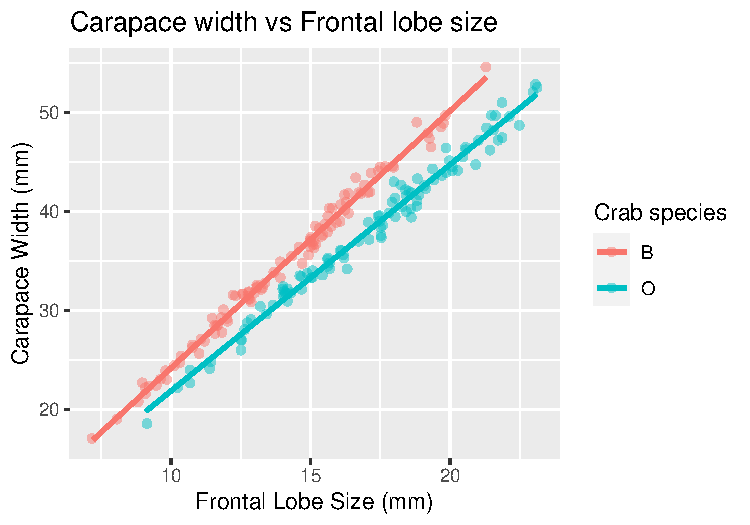
\includegraphics{CrabProject_files/figure-latex/figure1-1} 

}

\caption{Spread of Front lobe size against Carapace width based on color}\label{fig:figure1}
\end{figure}

This plot shows that blue crabs on average have wider carapaces and
shorter frontal lobes. This could be a good indicator to determine the
subspecies of the crab.

\begin{figure}[H]

{\centering 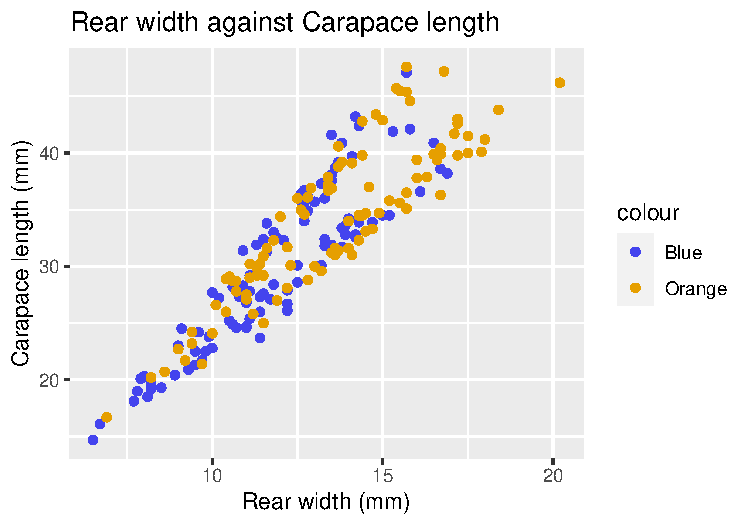
\includegraphics{CrabProject_files/figure-latex/figure2-1} 

}

\caption{Spread of Rear width against Carapace length based on color}\label{fig:figure2}
\end{figure}

This plot does not show a clear difference between blue and orange
crabs. Still there are 2 separated groups, this could be investigated
further.

\begin{figure}[H]

{\centering 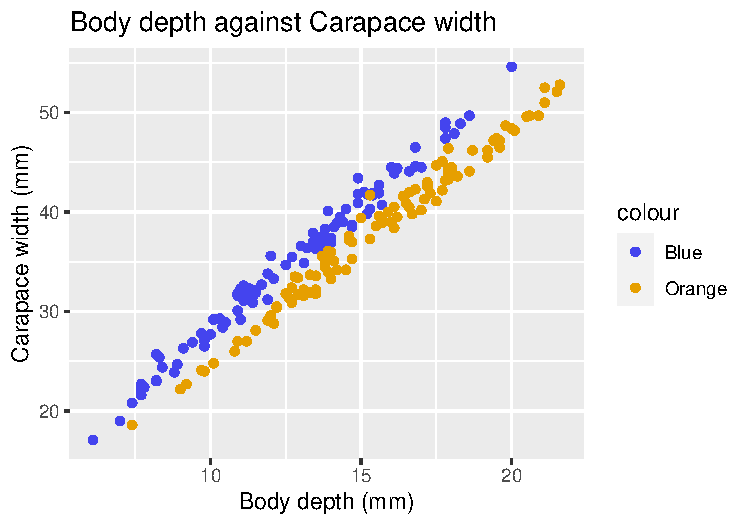
\includegraphics{CrabProject_files/figure-latex/figure3-1} 

}

\caption{Spread of Body depth against Carapace width based on color}\label{fig:figure3}
\end{figure}

This plot shows again that blue crabs on average have wider carapaces,
but that orange crabs tend to have deeper bodies. This could also be a
good indicator to determine the subspecies of the crab, though its less
clear than figure 1.

As shown in the figures one and three, the metrics of the orange and the
blue crabs are in two separate groups. This could mean that the two
species could be identifiable by their carapace width. However, figure
two also has two clear groups but the colors of the crabs are mixed.
This could mean that these two groups are separated by gender.

\begin{figure}[H]

{\centering 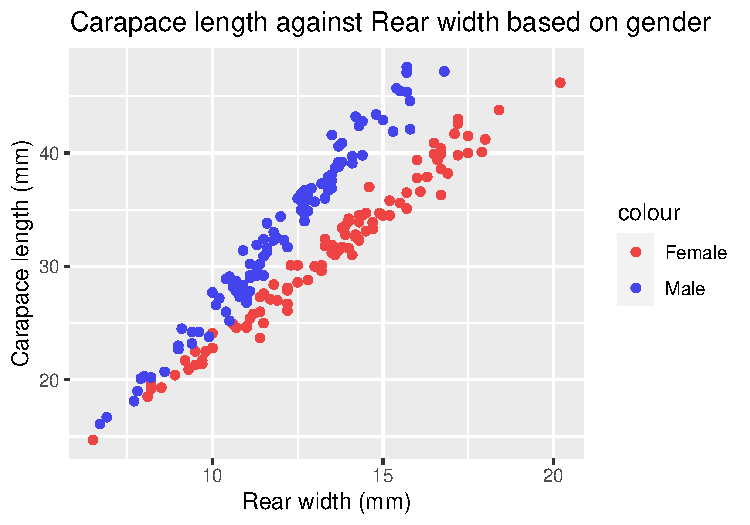
\includegraphics{CrabProject_files/figure-latex/figure4-1} 

}

\caption{Spread of Carapace length against Rear width based on gender}\label{fig:figure4}
\end{figure}

As shown in figure 4, it is indeed two groups of the genders of the
crabs. This means that the males have longer carapaces than the females.
The difference in carapace length for both genders are explored further.

\begin{figure}[H]

{\centering 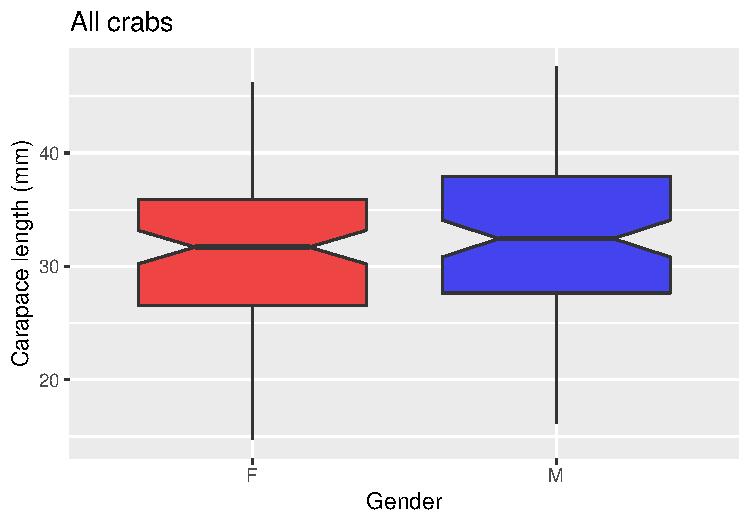
\includegraphics{CrabProject_files/figure-latex/figure5-1} 

}

\caption{Distribution of Carapace length for all male and female crabs}\label{fig:figure5}
\end{figure}

This plot does not show a big difference between male and female crabs.
The female crabs have a slightly shorter carapace, but it does not seem
significant. This could be investigated further, but is not much
connected to the research question.

\begin{figure}[H]

{\centering 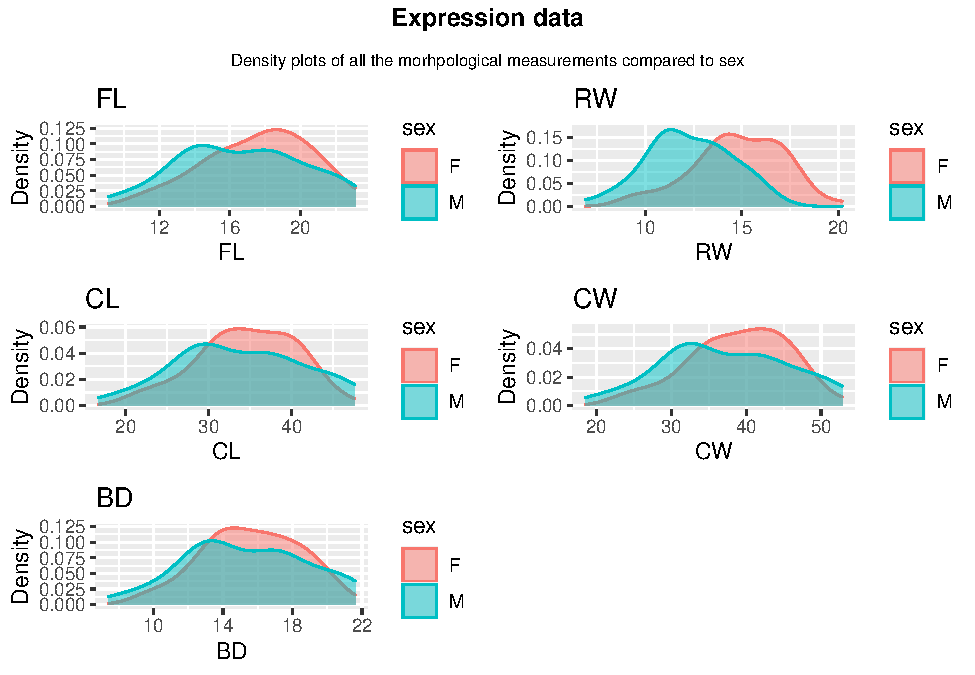
\includegraphics{CrabProject_files/figure-latex/figure6-1} 

}

\caption{Distribution of Carapace length for the orange and the blue male and female crabs}\label{fig:figure6}
\end{figure}

Figure 6 shows a small difference in the length of the carapace between
male and female orange crabs. It shows that the male crabs have on
average a shorter carapace, but the difference is not that big. Figure 7
shows a bigger difference in the length of the carapace between male and
female blue crabs. Here, the difference in means does seem significant.

As shown in figure 7, it is mainly the blue crabs that have a
significant difference in carapace length between genders. It shows that
the male crabs have longer carapace lengths on average. In figure 6 its
clear that the male orange crabs have shorter carapace lengths on
average compared to the females.

A variables PCA plot was generated to see how correlated all the
variables are.

\begin{center}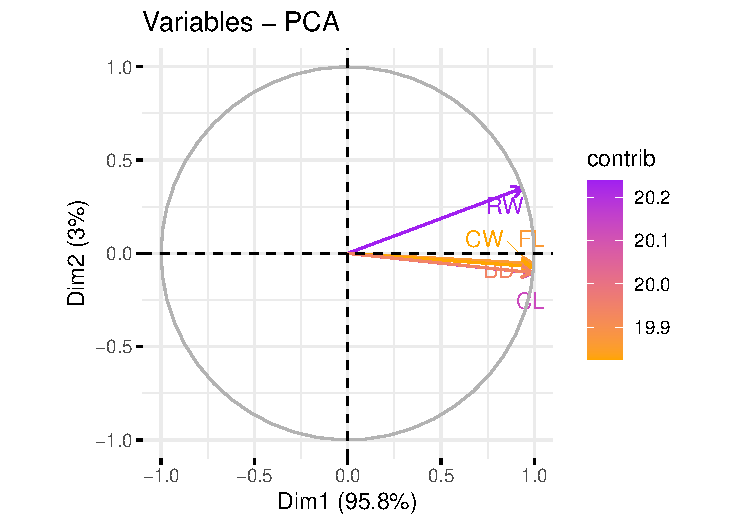
\includegraphics{CrabProject_files/figure-latex/pca-1} \end{center}

This PCA plot shows that the variables are highly correlated. The least
correlated variable is the Rear width. This vector has the largest angle
with the Carapace length, the same two variables were used to discover
the difference in carapace length distribution between the genders.

\hypertarget{cleaning-of-the-data}{%
\subsection{Cleaning of the data}\label{cleaning-of-the-data}}

In its current form, the data is not ready for machine learning. Because
of the id column, some of the machine learning algorithms overfit their
model by using this column. So this column should be removed first. The
species columns was also moved to the last column so it would be used as
the class attribute.

\hypertarget{machine-learning}{%
\subsubsection{Machine learning}\label{machine-learning}}

To find out what machine learning algorithm is the best for predicting
the species of crab, multiple algorithms were tested. These algorithms
are ZeroR, OneR, Simple logistic, Naive bayes, Random forest, J48, SMO
and K-nearest neighbor. These algorithms were tested using 10 fold
cross-validation. The highest quality metric for this dataset is the
accuracy, since it does not matter whether a blue crab is predicted to
be orange, or an orange crab to be blue. The software used to calculate
the accuracy is weka. After the classification, the accuracy of these
algorithms was saved in a csv file, and are shown in this barplot below.

\begin{figure}[H]

{\centering 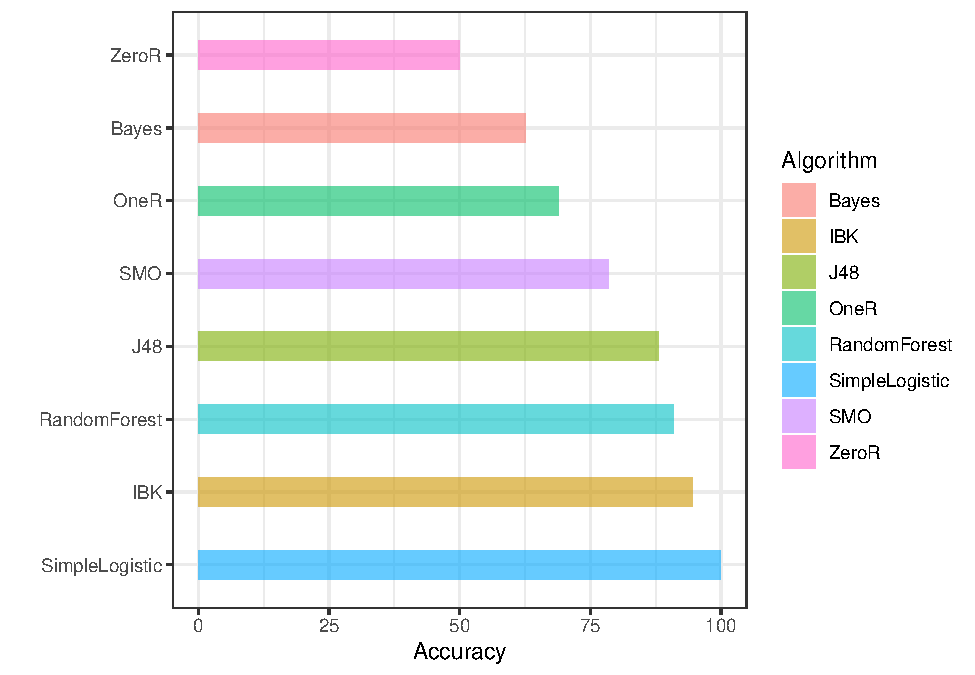
\includegraphics{CrabProject_files/figure-latex/ml-1} 

}

\caption{The accuracy of the machine learning algorithms ordered from low to high.}\label{fig:ml}
\end{figure}

This plot shows a few interesting things, most notably the 100\%
accuracy of Simple logistic. The output in weka of the classification
using Simple logistic with 10 fold cross-validation shows a model for
each species. The model for the blue crabs shows 1.03 + {[}FL{]} * -0.6
+ {[}CW{]} * 0.31 + {[}BD{]} * -0.22. The model for the orange crabs
shows -1.03 + {[}FL{]} * 0.6 + {[}CW{]} * -0.31 + {[}BD{]} * 0.22. The
values in the model of the orange crabs are the values of the model of
the blue crabs times -1. The metrics used in the models are Front lobe
size, Carapace width and Body depth. The barplot also shows an exact
50\% accuracy for the ZeroR algorithm. This is expected since the data
has the same amount of blue crabs as orange crabs.

Using the output from the simple logistic algorithm, the following roc
curve can be made.

\begin{center}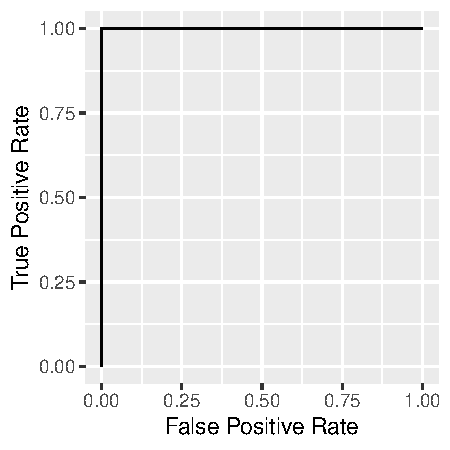
\includegraphics{CrabProject_files/figure-latex/roc-1} \end{center}

The curve is of course two straight lines because the accuracy is 100\%.

\newpage

\hypertarget{conclusion-discussion}{%
\section{Conclusion \& Discussion}\label{conclusion-discussion}}

The goal was to get the dataset ready for machine learning. The data was
analyzed and cleaned to make so it is ready to be used in machine
learning algorithms. The data does not contain many outliers. The data
points seem easy to classify since most plots show clear groups of blue
and orange crabs. As shown in figure 4, the gender of the crab could
also be a good attribute to help predict the species of crab. The data
also had to be cleaned. This was done by removing the index column,
since this column can not be used to help determine the species of crab.
It might also be a problematic attribute for some machine learning
algorithms. Then, the species column was moved to the last column, so
the machine learning algorithms will use this column as the class index.

\hypertarget{future-work-proposal}{%
\section{Future work proposal}\label{future-work-proposal}}

Future research can be used to show more correlation between other
measurements. It can be researched whether or not the gender of the crab
could be predicted using these morphological measurements. Machine
learning use could also be improved by expanding the dataset, or getting
different amounts of blue or orange crabs, with different amounts of
male and female crabs.

\newpage

\hypertarget{sources}{%
\section{Sources}\label{sources}}

\hypertarget{references}{%
\subsection{References}\label{references}}

{[}1{]} Campbell, N.A. and Mahon, R.J. (1974) A multivariate study of
variation in two species of rock crab of genus Leptograpsus. Australian
Journal of Zoology 22, 417--425.

\hypertarget{github-repositories}{%
\subsection{Github repositories}\label{github-repositories}}

Link to the report and log repository:
\url{https://github.com/IJsbarnd/CrabWrapper}

Link to the java wrapper repository:
\url{https://github.com/IJsbarnd/thema9_2}

\end{document}
